\section{数据处理不等式}
\label{sec:info-data-processing}

观测$Y$含有关于$X$的信息$I(X;Y)$。实际中观测很少原样使用：读数会被四舍五入，记录会被压缩，信号会再经过一段有噪声的线路。处理后得到$Z$，它含有的关于$X$的信息能否比$Y$多？如果处理时只用了$Y$，没有再接触$X$的任何来源，答案应当是否定的。本节把“只用了$Y$”写成条件独立，再用互信息的链式法则证明这个直觉，并研究什么时候处理不损失信息。

\subsection{后处理的信息损失}
\label{sec:info-dpi-loss}

“$Z$只依赖$Y$”有两种说法。一种是生成方式：先有$(X,Y)$，再按一个只以$y$为输入的随机规则$K(y,\cdot)$产生$Z$，这个规则不看$X$。另一种是条件独立：$X\perp\!\!\!\perp Z\mid Y$。第~\ref{chap:conditional-distributions}章证明了两种说法在标准Borel空间上等价。满足这个条件时，称$X,Y,Z$构成\term{Markov链}（Markov chain），记作$X\to Y\to Z$。确定性处理$Z=g(Y)$是特例，规则$K(y,\cdot)$是点质量。

\begin{theorem}[数据处理不等式]
\label{thm:info-data-processing}
设$X,Y,Z$取值于标准Borel空间，$X\to Y\to Z$。则
\begin{equation}
  I(X;Z)\leq I(X;Y).
  \label{eq:info-data-processing}
\end{equation}
\end{theorem}

\begin{proof}
用链式法则~\eqref{eq:info-mi-chain-rule}按两种顺序展开$I(X;Y,Z)$。先$Y$后$Z$：
\[
  I(X;Y,Z)=I(X;Y)+I(X;Z\mid Y)=I(X;Y),
\]
其中$I(X;Z\mid Y)=0$由条件独立与定理~\ref{thm:info-conditional-mi-zero}得到。先$Z$后$Y$：
\[
  I(X;Y,Z)=I(X;Z)+I(X;Y\mid Z)\geq I(X;Z),
\]
因为条件互信息非负。两式合并即得式~\eqref{eq:info-data-processing}。整个论证只是非负量的相加和比较，在$[0,+\infty]$中进行，不需要任何熵有限。
\end{proof}

式~\eqref{eq:info-data-processing}称为\term{数据处理不等式}（data processing inequality）。证明还给出了损失的大小。若$I(X;Y)<\infty$，两种展开相等，移项得到
\begin{equation}
  I(X;Y)-I(X;Z)=I(X;Y\mid Z).
  \label{eq:info-dpi-gap}
\end{equation}
处理损失的信息，正是已知$Z$以后$Y$还能提供的关于$X$的信息。

\paragraph{两个例子}
图~\ref{fig:info-markov-chain}(a)是确定性的合并。$X$在$\{0,1,2,3\}$上均匀，$Y=X$，$Z=\lfloor Y/2\rfloor$把$0,1$并成$0$，把$2,3$并成$1$。由定理~\ref{thm:info-mi-entropy}，
\[
  I(X;Y)=H(X)=\ln4,\qquad I(X;Z)=H(Z)=\ln2.
\]
合并丢掉了“在组内是哪一个”这一位信息，损失$I(X;Y\mid Z)=\ln2$。

\begin{BookInlineFigure}
  \centering
  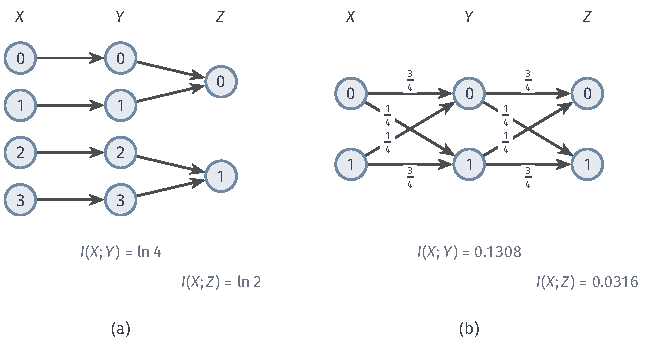
\includegraphics[width=110.1mm]{figures/07-probability/04-distribution-analysis/tikz/info-markov-chain/figure.pdf}
  \caption{两条Markov链$X\to Y\to Z$，箭头为转移概率。(a)$X$在四个标签上均匀，$Y=X$，$Z=\lfloor Y/2\rfloor$合并相邻标签。(b)公平硬币$X$经两段独立的线路，每段以概率$\tfrac14$翻转。下方为与$X$的互信息（nat）。}
  \label{fig:info-markov-chain}
\end{BookInlineFigure}

图~\ref{fig:info-markov-chain}(b)是添加独立噪声。$Y$是$X$经以概率$\tfrac14$出错的线路得到的，$Z$是$Y$再经一段独立的、以概率$\varepsilon_2$出错的线路得到的。$Z\neq X$当且仅当恰好一段出错，所以$X$到$Z$的总出错概率是
\[
  \tfrac14(1-\varepsilon_2)+\tfrac34\varepsilon_2.
\]
$\varepsilon_2=\tfrac14$时为$\tfrac38$，于是
\[
  I(X;Z)=\ln2-h_{\mathrm{b}}(\tfrac38)\approx0.0316<I(X;Y)\approx0.1308.
\]
图~\ref{fig:info-dpi-cascade}画出$I(X;Z)$随$\varepsilon_2$的变化：第二段线路越不可靠，剩下的信息越少，$\varepsilon_2=\tfrac12$时降为零。无论第二段怎样设计，曲线都不会越过$I(X;Y)$。

\begin{BookInlineFigure}
  \centering
  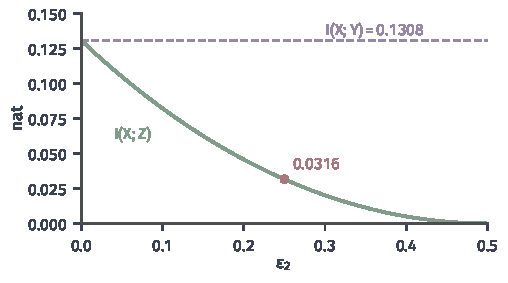
\includegraphics[width=86mm]{figures/07-probability/04-distribution-analysis/matplotlib/info-dpi-cascade/figure.pdf}
  \caption{两段串联线路。第一段翻转概率$\tfrac14$，第二段为$\varepsilon_2$。绿线为$I(X;Z)$，紫虚线为$I(X;Y)\approx0.1308$，单位nat；红点为$\varepsilon_2=\tfrac14$时的$0.0316$。}
  \label{fig:info-dpi-cascade}
\end{BookInlineFigure}

\paragraph{两个推论}
取$Z=g(Y)$为任意可测函数，得到$I(X;g(Y))\leq I(X;Y)$：任何对观测的计算都不能增加关于$X$的信息。再取离散的$X$并令$Y=X$，联合质量$p_{X,g(X)}(x,g(x))=p_X(x)$，代入式~\eqref{eq:info-mutual-information-discrete}，比值是$1/p_{g(X)}(g(x))$，所以$I(X;g(X))=H(g(X))$，特别地$I(X;X)=H(X)$。于是
\[
  H(g(X))\leq H(X).
\]
对离散变量作函数变换只会合并取值，熵不增；$g$是单射时取等号。注意微分熵没有这个性质，式~\eqref{eq:info-differential-entropy-scale}中$\lvert a\rvert>1$时$h(aX)>h(X)$。

\paragraph{条件独立的作用}
定理的前提不能去掉。仍看图~\ref{fig:info-markov-chain}(b)的第一段：$Y=X\oplus N$，$N$是翻转噪声。若处理者碰巧知道$N$，令$Z=Y\oplus N$，则$Z=X$，$I(X;Z)=\ln2$，远大于$I(X;Y)$。这里$Z$不只依赖$Y$，还依赖与$X$在给定$Y$时相关的$N$：给定$Y=y$时，$N=0$当且仅当$X=y$。所以$X\perp\!\!\!\perp Z\mid Y$不成立。“只用了$Y$”的确切意思是：处理中引入的额外随机性，在给定$Y$时与$X$独立。

条件独立是对称的：$X\perp\!\!\!\perp Z\mid Y$等价于$Z\perp\!\!\!\perp X\mid Y$，所以$X\to Y\to Z$也是$Z\to Y\to X$，同样有$I(X;Z)\leq I(Y;Z)$。箭头只是书写习惯。Markov链描述的是联合分布的一种结构，信息在其中两端都要经过$Y$；它并不规定哪个变量产生了哪个变量。同一个联合分布既可以由“$X$经过线路得到$Y$”产生，也可以由“先抽$Y$、再按后验抽$X$”产生，不等式对两者相同。

\subsection{信息保留}
\label{sec:info-dpi-preservation}

数据处理不等式什么时候取等号？最简单的情形是处理可以撤销。设$Z=g(Y)$，其中$g$是可测双射，逆映射也可测。则$X\to Y\to Z$，同时$Y=g^{-1}(Z)$，又有$X\to Z\to Y$。对两条链分别应用定理~\ref{thm:info-data-processing}，得到
\[
  I(X;Z)\leq I(X;Y)\leq I(X;Z),
\]
所以$I(X;g(Y))=I(X;Y)$。对两个变量分别作这样的变换，互信息都不变；这与微分熵随坐标改变形成对比。

可逆是充分条件，不是必要条件。设$X$是公平硬币，$U$是与$X$独立的公平硬币，观测$Y=2X+U\in\{0,1,2,3\}$，处理为$Z=\lfloor Y/2\rfloor$。$Z=X$，所以
\[
  I(X;Z)=H(X)=\ln2.
\]
另一方面，$X$是$Y$的函数，$I(X;Y)=H(X)-H(X\mid Y)=\ln2$。处理把四个值并成两个，不可逆，却没有损失任何关于$X$的信息：被丢掉的$U$与$X$无关。

一般的判据由式~\eqref{eq:info-dpi-gap}给出。

\begin{theorem}[信息保留的条件]
\label{thm:info-dpi-equality}
设$X,Y,Z$取值于标准Borel空间，$X\to Y\to Z$，并且$I(X;Y)<\infty$。则$I(X;Z)=I(X;Y)$当且仅当$X\perp\!\!\!\perp Y\mid Z$，即$X\to Z\to Y$也成立。
\end{theorem}

\begin{proof}
由式~\eqref{eq:info-dpi-gap}，等号当且仅当$I(X;Y\mid Z)=0$，再由定理~\ref{thm:info-conditional-mi-zero}，这等价于$X\perp\!\!\!\perp Y\mid Z$。
\end{proof}

$X\to Z\to Y$说的是：知道$Z$以后，$Y$中剩下的部分与$X$无关。上面的例子中，给定$Z=X$以后，$Y$只多出一个独立的$U$，确实与$X$条件独立。在图~\ref{fig:info-markov-chain}(a)中，给定$Z=0$时$Y$在$\{0,1\}$中仍随$X$变化，条件独立不成立，信息有损失。

定理要求$I(X;Y)<\infty$，因为式~\eqref{eq:info-dpi-gap}要移项。互信息为无穷时，$I(X;Z)=I(X;Y)=\infty$可以与“有损失”同时出现。设$X\sim\operatorname{Unif}(0,1)$，$Y=X$，$Z$由$X$二进制展开的奇数位组成。$Z$本身服从无原子的分布，并且是$X$的函数，与第~\ref{sec:info-mi-definition}节的对角线论证相同，联合分布集中在一个函数图像上，而边缘乘积给这个图像零概率，所以$I(X;Z)=+\infty=I(X;Y)$。但给定$Z$以后，$X$的偶数位仍是独立均匀的，$Y=X$与$X$之间还有无穷多的信息，$I(X;Y\mid Z)=+\infty$。两边都是无穷，比较互信息的数值已经看不出损失，要直接看条件互信息。
